% !TeX root = ../main.tex

\chapter{基于柄圈的网格切割算法}

\section{简介}

\citet{oncomputinghantun} 基于几何直观,发现曲面网格的“把手”和“通道”等特征对于拓扑简化和特征检测都很有帮助,因此提出了柄圈和其形式化定义。在此基础上,\citet{Chai2018}认为柄圈是最短割缝问题的一个好的启发,并且实现了基于柄圈进行曲面切割的方法。

直观上,柄圈和通道圈描述了曲面的一些几何特征,这些特征可以用来切割曲面。图 \ref{fig:hantuncadgadget} 展示了一个 CAD 工件上的一些柄圈和通道圈。

\begin{figure}[h]
    \centering
    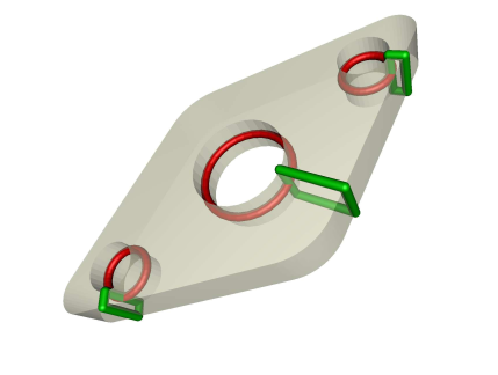
\includegraphics[width=0.5\textwidth]{hantun-cad-gadget.png}
    \caption{CAD 工件:红色圈为通道圈,绿色圈为柄圈}
    \label{fig:hantuncadgadget}
    \note{图片源自 \citet{oncomputinghantun}}
\end{figure}

本节首先介绍柄圈形式化描述所需要的基本知识,即单纯同调论和 $ \mathbb{Z}_2 $ 系数域下同调论描述的几个群的基表示,然后再给出计算 $ H_1(K; \mathbb{Z}_2) $ 的最优基的算法。之后,本节会介绍柄圈的形式化定义,以及一个基于前述算法的、计算柄圈的算法。

\section{单纯同调论}

单纯同调论 (Simplicial homology) 是描述欧氏空间中具有组合结构的空间的同调论。根据其研究的主要方法,单纯同调论又被称为组合拓扑学。本节更详细的内容可以参考\cite{jctpxjy}。

$ R_n $ 中处于一般位置的 $ n + 1 $ 个点 $ \{a_0, \dots, a_n\} $ ($n > 0$)的凸组合被称为一个 $ n $ 维单纯形,简称 n-单形,记作 $ (a_0, a_1, \dots, a_n) $。称 $ a_i$ 为其顶点。

设 $ K $ 为以单形为元素的有限集合,如果 $ K $ 满足
\begin{enumerate}
    \item $ K $ 中任意两个 $m$-单形交集为空集,或相交部分为某个在 K 中的 $m-1$-单形
    \item 构成 $ m$-单形顶点组成的 $ m - 1 $-单形仍在 $ K $ 中
\end{enumerate}
则称 $ K $ 为单纯复合形,又称为单复形。复形中所有维度不超过 $ m $ 的单形构成 $ K $ 的子复形,称为 $ K $ 的 m-骨架,记作 $ K^m $。

可以看出,单复形可以表示欧氏空间的一个子集,如果有这样的子集 $ X $ 可以被单复形中的所有单形的并表示,则成这样的 $ X $ 为多面体。显然,我们研究的网格就是这样的多面体。

为了构造同调群,我们还需要引入定向单形的概念。定向单形为取定了定向的单形,此时单形分为相同和相反的两种定向,这两种定向在稍后定义的链群中互为逆元。形式上的说,即考虑 m-单形 $ (p_0, p_1, \dots, p_m) $,则 
$$ p_{i_0} p_{i_1} \dots p_{i_m} = sgn(P) p_{0} p_{1} \dots p_{m} $$
其中 $ P $ 为 $ \{0, 1, 2, \dots, m \} $ 到 $ \{i_0, i_1, i_2, \dots, i_m \} $ 的一个排列,$ sgn(P) $ 为此排列的符号。

$ K $ 中所有 m-单形所对应的 m-定向单形所生成的在 $ \mathbb{Z} $ 系数域上的自由阿贝尔群称为 m-链群,记作 $ C_m(K) $。$ C_m(K) $ 的元素称为 m-链。为了叙述上的方便,定义 $ m < 0 $ 或者 $ m > \dim K $ 时 $ C_m(K) = 0 $。

定义边缘算子 $ \partial_q: T_q(K) \to C_{q-1}(K) $ 满足 
$$ \partial_q (a_0 a_1 \dots a_q) = \sum_{i=0}^{q} (-1)^i a_0 \dots \hat{a_i} \dots a_q $$

其中  $ \hat{a_i} $ 表示删除 $ a_i $,$ T_q(K) $ 为 $ K $ 的所有 q-定向单形的集合。可以看出,边缘算子描述了一个单形组合和其对应的“边界”的关系。同时可以证明,$ \partial q $ 在满足 $\partial_q(-s) = -\partial_q(s) $ 的情形下可以唯一的扩张为 $ C_q(K) \to C_{q-1}(K) $ 的同态。为了方便,此同态仍然记作 $ \partial_q $,则有
$$
\partial_q (\sum_i n_i s_i) = \sum_i n_i \partial_q (s_i)
$$
成立。

在考虑边缘同态的过程中,我们可以自然的得到 $ C_q(K) $ 的两个子群 $ Z_q(K) = ker(\partial_q(K)) $ 和 $ B_q(K) = Im(\partial_{q+1}(K)) $,分别称为 n-闭链群和 n-边缘链群。$ Z_q(K) $ 中的元素称为 n-闭链。显然,$ Z_q(K) $ 和 $ B_q(K) $ 都是自由阿贝尔群。同时可以证明,$ B_q(K) $ 是 $ Z_q(K) $ 的子群,这可以由下面的事实得到($ c \in C_q(K) $):
\begin{align*}
\partial_{q-1} (\partial_q (c)) &= \partial_{q-1} (\sum_{i=0}^q (-1)^i a_0 a_1 \dots \hat{a_i} \dots a_q) \\
&= \sum_{i=1}^q (-1)^i \partial_{q-1} (a_0 a_1 \dots \hat{a_i} \dots a_q) \\
&= \sum_{i=1}^q (-1)^i ( \sum_{j=1}^{i-1} (-1)^j a_0 \dots \hat{a_j} \dots \hat{a_i} \dots a_q + \sum_{j=i+1}^{q} (-1)^{j-1} a_0 \dots \hat{a_i} \dots \hat{a_j} \dots a_q ) \\
&= \sum_{0 \le j < i \le q} (-1)^{i+j} a_0 \dots \hat{a_j} \dots \hat{a_i} \dots a_q - \sum_{0 \le i < j \le q} (-1)^{i+j} a_0 \dots \hat{a_i} \dots \hat{a_j} \dots a_q \\
&= 0
\end{align*}

既然 $ B_q(K) $ 是 $ Z_q(K) $ 的子群,又因为 $ B_q(K) $ 是阿贝尔群,所以 $ B_q(K) $ 是正规子群。于是,我们定义q-同调群 $ H_q(K) $ 为 $ Z_q(K) / B_q(K) $,即 $ Z_q(K) $ 对 $ B_q(K) $ 的商群。如果 $ K $ 中两个闭链 $ c $,$ c' $属于同一个 $ H_q(K) $ 确定的等价类,则称这两个闭链同调,记为 $ c \sim c' $。

由于 $ Z_q(K) $ 和 $ B_q(K) $ 在 $ K $ 为有限集时均为有限生成自由阿贝尔群,则他们的商群也是有限生成阿贝尔群。由有限生成阿贝尔群的分类定理,可以将群分为自由子群和扭子群的直和:
$$
H_q(K) \simeq \underbrace{Z \oplus Z \oplus \dots \oplus Z}_{b_q(K)} \oplus Z_{i_1} \oplus \dots \oplus Z_{i_m}
$$

其中 $ b_q(K) $ 被称为 $ K $ 的 $ q $ 维 Betti 数。

我们在前面的推导过程中对链群使用的系数域为 $ \mathbb Z $。如果我们将 $ \mathbb{Z} $ 换为 $ \mathbb{Z}_2 $ 或 $ \mathbb{R} $,由于 $ \mathbb{Z}_2 $ 和 $ \mathbb{R} $ 均没有非平凡的扭子群,那么 $ H_q(K; Z_2) $ 或 $ H_q(K; R) $ 的结构就很容易得到:
$$
H_q(K;\mathbb{R}) \simeq H_q(K;\mathbb{Z}_2) \simeq\underbrace{Z \oplus Z \oplus \dots \oplus Z}_{b_q(K)}
$$

所以 $ b_q(K) $ 又可以写作 $ \dim H_q(K; \mathbb{R}) $ 。由此,我们也可以得到在 $ \mathbb{Z}_2 $ 下 $ C_q(K) $,$ Z_q(K) $,$ B_q(K) $ 和 $ H_q(K) $ 均为线性空间,有维度和基的概念。

\section{闭曲面分类}

闭曲面,即没有边界点的紧致连通曲面。我们处理的网格,由于其分片线性表示的特点而天然具有紧致性,故代数拓扑中研究的闭曲面的拓扑类型对于网格处理中拓扑类型的讨论有很大帮助。

我们称环柄为环面上挖一个洞后形成的空间, $ \{nT^2\} $ 即球面上安 $ n $ 个环柄所得空间。在球面上挖一个洞,并在洞口粘结 Mobius 带,这种操作称为在球面上安交叉帽。$ \{mP^2\} $ 即安了 $ m $ 个交叉帽的球面。可以证明,$ \{nT^2\} $ 为亏格为 $ n $ 的可定向闭曲面,而 $ \{mP^2\} $ 为亏格为 $ m $ 的不可定向闭曲面。

事实上,我们有以下定理:

\begin{theorem}
    (\emph{闭曲面分类定理})~
    $ \{nT^2 \} $ 和 $ \{mP^2\} $ 不重复地列出了闭曲面的所有拓扑类型。
\end{theorem}

这个定理因为其重要性,历史上有很多证明,一个简单的证明可以参考\cite{jctpxjy}。这样,我们讨论 $ nT^2 $ 类型的拓扑空间时,大多数时候只要证明其在 n-环面的某个三角剖分上成立即可。

\section{一维链,闭链,边缘链和同调群的基表示}

下面的讨论均在 $ \mathbb{Z}_2 $ 域下进行。值得注意的是,$ \mathbb{Z}_2 $ 下 $ -1 = 1 $,所以单形的定向在此空间下只有一种,圈、路径等 $ C_m(K) $ 中的元素也不需要指明定向。

一维链群在 $ \mathbb{Z}_2 $ 下的线性空间表示很好得到,其中 $ c_i $ 为边 $ e_i $ 对应的系数。
$$
c = \begin{bmatrix}
        c_1 \\
        c_2 \\
        \cdots \\
        c_{|E|} \\
    \end{bmatrix} \in C_1(K) \quad (c_i \in \{0, 1\})
$$

$ C_1(K) $ 的(自然)基为 $ (e_1, \dots, e_{|E|}) $,其中 $ e_i $ 为 $ K $ 的 1-骨架 $ K^1 $ 的第 $ i $ 条边。

考虑 $ K^1 $ 的某个生成树 $ T $,则有 $ |V| - 1 $ 条边在生成树上, $ |E| - |V| + 1 $ 条边不在生成树上。对于不在生成树上的边 $ e_{m_i} $,生成树提供了从边的一个端点到另一个端点的路径,这个路径连同 $ e_{m_i} $ 形成一个圈,记为 $ \gamma(T, e_{m_i}) $。

这样,我们得到了 $ \{ \gamma(T, e_{m_1}), \dots, \gamma(T, e_{m_{k}}) \} $,其中 $ k = |E| - |V| + 1 $。$ \gamma(T, e_{n_i}) $ 和 $ \gamma(T, e_{n_j}) $ 间线性无关,因为 $ e_{n_j} \in \gamma(T, e_{n_i}) $ 当且仅当 $ i = j $。

对于一个任意圈 $ z $,固定树 $ T $ 上的某个顶点 $ s $,记 $ T[s, u] $ 为树上 $ s $ 到 $ u $ 的唯一路径,那么
$$
z = \sum_{e=uv \in z} e = \sum_{e=uv \in z} (T[s, u] + e + T[s, v]) = \sum_{e \in z} \gamma(T, e)
$$

其中第三个等号成立是因为所有在树上的边的 $ T[s, u] + e + T[s, v] = 0 $。由此,我们可以看出,$ \{ \gamma(T, e_{m_1}), \dots, \gamma(T, e_{m_{k}}) \} $ 构成 $ Z_1(K) $ 的一组基,矩阵表示如下:
$$
Z = 
\begin{bmatrix}
\begin{array}{c|c|c}
    \gamma(T, e_{m_1}) & \cdots & \gamma(T, e_{m_{k}})
\end{array}
\end{bmatrix}
$$

为了方便,我们引入优先基的概念。给定秩为 $ r $ 的矩阵 $ A $,由 $ A $ 的部分列向量组成的 $ B_{opt} = \{a_{i_1}, \dots, a_{i_r}\} $ 被称为优先基,如果 $ \{ i_1, \dots, i_r \} $ 是让 $ {\rm rank}(B_{opt}) = {\rm rank}(A) $ 的,在标号顺序上最小的一组指标集。记 $ {\rm EarliestBasis}(A) $ 为 $ A $ 的优先基 $ B_{opt} $。

那么,$ B_1(K) $ 的基可以用如下表示,记为 $ B $:
$$
B = 
{\rm EarliestBasis}(\begin{bmatrix}
    \begin{array}{c|c|c}
    \partial_1(f_1) & \cdots & \partial_1(f_{|F|})
\end{array}
\end{bmatrix})
$$

考虑到 $ H_1(K) = Z_1(K) / B_1(K) $,那么
$$
\begin{bmatrix}
    \begin{array}{c|c}
        B & H
    \end{array}
\end{bmatrix} =
{\rm EarliestBasis}(\begin{bmatrix}
    \begin{array}{ccc|c}
        \partial_1(f_1) & \cdots & \partial_1(f_{|F|}) & Z
    \end{array}
\end{bmatrix})
$$

这是因为 $ \dim H_1 = \dim Z_1 - \dim B_1 $,而 $ \dim B_1 = {\rm rank}(B) $,所以剩下的 $ {\rm rank}(Z) - {\rm rank}(B) $ 个列向量就是 $ H $ 的基了。

$ H $ 的维数在闭曲面且为 $ nT^2 $ 类型时也被称为亏格,用 $ g $ 表示。此时,$ g $ 和欧拉特征数 $ \chi(K) = |V| - |E| + |F| $ 满足关系 $ \chi(K) = 2 - 2g $,此关系是 Euler-Poincare 公式的自然结论。

有了 $ H $ 的基,我们就可以为每个圈都计算对应的坐标,即同调向量 (homology vector) 了。

\section{计算最短同调圈}
\label{sec:shortest-h1m}

\citet{Busaryev2012} 提出了利用标注 (annotation) 在 $ O(n^\omega + n^2 g^{\omega - 1}) $ 时间复杂度下计算 $ H_1(K; \mathbb{Z}_2) $ 的最优基的算法。

所谓最优基,就是对任意 $ c = \sum_i c_i s_i \in Z_1(K) $,定义 $ w(c) = \sum_i c_i w(s_i) $ 为闭链 $ c $ 的权,并且求一组 $ H_1(K; \mathbb{Z}_2) $ 的基使得 $ \sum_{c} w(c) $ 最小。

算法的主要思路是,在曲面上按权重从短到长排序的圈中,挑选出前 $ 2g $ 个彼此互相不同调的圈构成的基,就是最优基。为了高效的计算,这里需要解决两个问题:
\begin{enumerate}
    \item 如何减少需要考虑的圈的数量?
    \item 如何快速判断两个圈彼此是否同调?
\end{enumerate}

\subsection{利用紧性质缩小搜索空间}

问题一的解决依赖 \citet{Erickson2005} 中提出的最优基的紧性质。当一个圈 $ l $ 包含 $ l $ 上任意的两点之间的最短路径时,称 $ l $ 具有紧性质。

\begin{proposition}
    (\citet{Busaryev2012})~
    每个 $ H_1(K; \mathbb{Z}_2) $ 的最优基中的圈都具有紧性质。
\end{proposition}
这个问题的证明可以参考 \cite{Busaryev2012}。
% \begin{proof}
%     首先,最优基中的每个圈都不能分解为一些更小的圈的并。假设可以分解为两个更小的圈,那一定有一个圈可以被被其它圈表示,则去掉该圈可以找到更优的基。

%     若圈 $ l_1 $ 不具有紧性质,取 $ x $ 和 $ y $ 是使得 $ l_1 $ 不包含 $ x $ 到 $ y $ 的最短路,则 $ l_1 $ 被分为两条从 $ y $ 到 $ x $ 的路,分别记为 $ \alpha $ 和 $ \beta $。记 $ \sigma $ 为 $ x $ 到 $ y $ 的最短路,则 $ l'_1 = \alpha \sigma $ 和 $ l''_1 = \beta \sigma $ 中至少有一个不能被其它圈的线性组合所表示,否则其不会出现在基中。由于 $ l'_1 $ 和 $ l''_1 $ 均比 $ l_1 $ 短,设不能被线性表示的圈为 $ l'_1 $,则我们找到了一组更优的基 $ l'_1, l_2, \dots l_{n} $。
% \end{proof}

记 $ T_s $ 为从顶点 $ s $ 开始的权函数意义下的最短路径树,即包含从 $ s $ 到任意点的最短路径的树。同时,记候选圈集合为
$$
\Pi = \bigcup_{s \in V} \{ \gamma(T_s, e) | e \in E \setminus E(T_s) \}
$$
我们有如下命题成立\cite{Busaryev2012}:
\begin{proposition}
    (\citet{Busaryev2012})~
    如果按权重升序排列 $ \Pi $ 中的圈,并且为每个圈计算同调向量,那么 $ {\rm EarliestBasis}(\Pi) $ 是 $ H_1(K; \mathbb{Z}_2) $ 的最优基。
\end{proposition}
原文\cite{Busaryev2012}将实现细节与证明混合在一起了,这里给出一个简化的证明:
\begin{proof}
    只要证明最优基中的圈一定在 $ \Pi $ 中。考虑每个圈 $ \gamma(T_s, e) $,其仅在 $ s $ 到任意一点 $ x \in \gamma(T_s, e) $ 时保留紧性质。事实上,每个紧的圈 $ l $都一定在某个 $ \gamma(T_s, e) $ 中,因为一定存在某个 $ s_i \in l $,且 $ \{\gamma(T_{s_i}, e_1), \dots, \gamma(T_{s_i}, e_{k})\} $ 生成了 1-闭链群,由于 $ l $ 的紧性质,$ l $ 一定为其中一个而不是其中某些的线性组合。因为最优基的圈一定是保留紧性质的圈,所以最优基的圈一定在 $ \Pi $ 中。
\end{proof}

通过以上命题,我们可以将候选的圈数量变为 $ O(|V|(|E|-|V|+1)) $ 。

\subsection{利用标注快速判断同调关系}
\label{subsec:annotation}

\citet{Busaryev2012} 中提出的标注方法可以帮我们解决问题二。

\begin{definition}
    一个 p-单形 的标注是一个函数 $ a: C_p(K) \to (\mathbb{Z}_2)^{g} $。两个 p-闭链 $ z $ 和 $ z' $ 彼此同调,当且仅当
    \begin{equation*}
        \sum_{\sigma \in z} a(\sigma) = \sum_{\sigma \in z'} a(\sigma)
    \end{equation*}
    此时,该 p-闭链的标注被定义为 $ a(z) = \sum_{\sigma \in z} a(\sigma) $。
\end{definition}

计算标注的方法如下所示:
\begin{enumerate}
    \item \emph{计算 $ Z_1(K) $ 的基}\quad 固定某个 $ K^1 $ 的生成树 $ T $,记 $ k = |E| - |V| + 1 $,$ E \setminus E(T) $ 的各边为 $ e_{m_1}, \dots, e_{m_k} $,则可以构造基 $ \{ \gamma(T, e_{m_1}), \dots, \gamma(T, e_{m_{k}}) \} $。
    \item \emph{计算 $ H_1(K) $ 的基}\quad 通过计算 $ {\rm EarliestBasis}([B | Z]) $ 并移除前 $ {\rm rank}(B) $ 列得到的剩余列向量,记为 $ H $,即为 $ H_1(K) $ 的基。同时,记 $ \tilde{Z} = [B | Z] $。
    \item \emph{计算标注}\quad 对每个圈 $ z = \gamma(T, e) $,其坐标是满足 $ \tilde{Z} x = z $ 的 $ x $ 的最后 $ {\rm rank}(Z) - {\rm rank}(B) $ 个分量,这些作为该圈的标注。我们令 $ E(T) $ 上的边对应的标注为零向量,令 $ E \setminus E(T) $ 上的边对应的标注为对应的圈的标注,这样就得到了所有边的标注。
\end{enumerate}

有了标注,我们只需要计算两个圈的标注是否相同,就可以判断两个圈是否同调了。这样,我们就解决了问题二。

\subsection{算法框架}

综上,我们可以得到算法的框架如下:

\begin{enumerate}
    \item 以任意一点为源点,计算生成树 $ T $,然后按照第\ref{subsec:annotation}节中的方法计算每个边的标注向量 $ a(z) $。
    \item 对 $ K $ 的每个顶点 $ s $:
    \begin{enumerate}
        \item 计算 $ s $ 出发的最短路径树,得到圈 $ \gamma(T_s, e_{m_1}), \dots, \gamma(T_s, e_{m_k}) $。
        \item 计算每个圈的权重和标注,并加入候选圈集合。
    \end{enumerate}
    \item 选出以总权重从小到大排列的候选圈的前 $ 2g $ 个彼此互相不同调的圈,即为要求的最优基。
\end{enumerate}

\section{计算柄圈}

\citet{oncomputinghantun} 在其文章中引入了柄圈 (handle loop) 和通道圈 (tunnel loop) 的概念。

考虑一个可定向闭曲面 $ \mathcal{M} $,将其放在一个三维球 $ S^3 $ 中,其将 $ S^3 $ 分为两部分。给定曲面的定向,我们称 $ S^3 \setminus \mathcal{M} $ 的两个连通片分别为内部和外部,分别记作 $ I $ 和 $ O $。我们定义
$$
\mathbb{I} = I \cup \mathcal{M}, \quad \mathbb{O} = O \cup \mathcal{M}
$$

那么,我们可以给出柄圈和通道圈的定义。

\begin{definition}
    $ c \in Z_1(M) $
    \begin{enumerate}
        \item $ c $ 是柄圈,如果 $ c \in B_1(\mathbb{I}) $ 且 $ c \notin B_1(\mathbb{O}) $
        \item $ c $ 是通道圈,如果 $ c \in B_1(\mathbb{O}) $ 且 $ c \notin B_1(\mathbb{I}) $
    \end{enumerate}
\end{definition}

我们观察到,如果我们沿着柄圈切割 $ \mathcal{M} $,并且将每个柄圈切割后剩下的“空洞”分别用两个圆盘补上,我们就可以“消灭”一个柄圈。这可以由以下命题以及闭曲面 $ nT^2 $ 的性质得到:

\begin{proposition}
    (\citet{oncomputinghantun})~
    对于亏格为 $ g $ 的可定向闭曲面 $ \mathcal{M} \subset S^3 $,存在 $ g $ 个柄圈 $ \{h_i\}_{i=1}^{g} $ 和 $ g $ 个通道圈 $ \{g_i\}_{i=1}^{g} $ ,分别构成 $ H_1(\mathbb{O}) $ 和 $ H_1(\mathbb{I}) $ 的基,且 $ \{h_i\}_{i=1}^{g} $ 和 $ \{t_i\}_{i=1}^{g} $ 构成 $ H_1(\mathcal{M}) $ 的一组基。
\end{proposition}

这个命题的证明可以参考 \citet{oncomputinghantun}。

考虑到第\ref{sec:shortest-h1m}节处计算最短同调圈的工作,我们是否可以通过求解 $ H_1(\mathcal{M}) $ 的一组基来计算 $ H_1(\mathbb{O}) $ 的基呢?答案是否定的,因为两个线性空间的直和的一组基并不一定能够直接拆分为两个线性空间各自的基。

不过,我们可以将其中的技术迁移到最短柄圈的计算上。我们只要:
\begin{enumerate}
    \item 对 $ H_1(\mathbb{O}) $ 进行三角剖分,得到单复形表示
    \item 求 $ H_1(\mathbb{O}) $ 的一组基,并且筛选时只选择在 $ H_1(\mathcal{M}) $ 上的圈
\end{enumerate}
就可以获得最短同调圈集 $ \{h_i\}_{i=1}^{g} $。

应用 $ \{h_i\}_{i=1}^{g} $,我们可以得到\citet{ShuangmingChaiThesis}工作中的基于柄圈的网格切割算法:
\begin{enumerate}
    \item 计算最短同调圈集 $ \{h_i\}_{i=1}^{g} $
    \item 构造割线集 $ C $ 为所有 $ h_i $ 之并,同时再加入任意两个相邻的边,应用该割线集进行切割
\end{enumerate}

这样,我们就可以得到多了 $ 2g $ 个洞的圆盘,我们将多余的洞补上就可以得到拓扑圆盘。